% !TEX TS-program = XeLaTeX
% use the following command: 
% all document files must be coded in UTF-8
\documentclass{textolivre}
% for anonymous submission
%\documentclass[anonymous]{textolivre}
% to create HTML use 
%\documentclass{textolivre-html}
% HTML compile using make4ht
% $ make4ht -c textolivre-html.cfg -u -x article "fn-in,svg,pic-align"   
%
% See more information on the repository: https://github.com/leolca/textolivre

% Metadata
\begin{filecontents*}{article.xmpdata}
    \Title{O uso da Wikiversidade no ensino do jornalismo científico: abertura, colaboração e conectivismo}
    \Author{Daniel Almeida Abrahão Dieb}
    \Language{pt}
    \Keywords{Jornalismo Científico \sep Wiki \sep Colaboração \sep Conectivismo \sep Abertura.}
    \Journaltitle{Texto Livre}
    \Journalnumber{1983-3652}
    \Volume{14}
    \Issue{1}
    \Firstpage{1}
    \Lastpage{25}
    \Doi{10.35699/1983-3652.2021.24935}

    \setRGBcolorprofile{sRGB_IEC61966-2-1_black_scaled.icc}
            {sRGB_IEC61966-2-1_black_scaled}
            {sRGB IEC61966 v2.1 with black scaling}
            {http://www.color.org}
\end{filecontents*}

% used in this example to provide source code environment
%\crefname{lstlisting}{lista}{listas}
%\Crefname{lstlisting}{Lista}{Listas}
%\usepackage{listings}
%\renewcommand\lstlistingname{Lista}
%\lstset{language=bash,
        breaklines=true,
        basicstyle=\linespread{1}\small\ttfamily,
        numbers=none,xleftmargin=0.5cm,
        frame=none,
        framexleftmargin=0.5em,
        framexrightmargin=0.5em,
        showstringspaces=false,
        upquote=true,
        commentstyle=\color{gray},
        literate=%
           {á}{{\'a}}1 {é}{{\'e}}1 {í}{{\'i}}1 {ó}{{\'o}}1 {ú}{{\'u}}1 
           {à}{{\`a}}1 {è}{{\`e}}1 {ì}{{\`i}}1 {ò}{{\`o}}1 {ù}{{\`u}}1
           {ã}{{\~a}}1 {ẽ}{{\~e}}1 {ĩ}{{\~i}}1 {õ}{{\~o}}1 {ũ}{{\~u}}1
           {â}{{\^a}}1 {ê}{{\^e}}1 {î}{{\^i}}1 {ô}{{\^o}}1 {û}{{\^u}}1
           {ä}{{\"a}}1 {ë}{{\"e}}1 {ï}{{\"i}}1 {ö}{{\"o}}1 {ü}{{\"u}}1
           {Á}{{\'A}}1 {É}{{\'E}}1 {Í}{{\'I}}1 {Ó}{{\'O}}1 {Ú}{{\'U}}1
           {À}{{\`A}}1 {È}{{\`E}}1 {Ì}{{\`I}}1 {Ò}{{\`O}}1 {Ù}{{\`U}}1
           {Ã}{{\~A}}1 {Ẽ}{{\~E}}1 {Ũ}{{\~u}}1 {Õ}{{\~O}}1 {Ũ}{{\~U}}1
           {Â}{{\^A}}1 {Ê}{{\^E}}1 {Î}{{\^I}}1 {Ô}{{\^O}}1 {Û}{{\^U}}1
           {Ä}{{\"A}}1 {Ë}{{\"E}}1 {Ï}{{\"I}}1 {Ö}{{\"O}}1 {Ü}{{\"U}}1
           {ç}{{\c{c}}}1 {Ç}{{\c{C}}}1
}


\journalname{Texto Livre: Linguagem e Tecnologia}
\thevolume{14}
\thenumber{1}
\theyear{2021}
\receiveddate{\DTMdisplaydate{2020}{08}{25}{-1}} % YYYY MM DD
\accepteddate{\DTMdisplaydate{2020}{10}{15}{-1}}
\publisheddate{\DTMdisplaydate{2021}{1}{4}{-1}}
% Corresponding author
\corrauthor{Daniel Almeida Abrahão Dieb}
% DOI
\articledoi{10.35699/1983-3652.2021.24935}
% Abbreviated author list for the running footer
\runningauthor{Dieb et al}
\editorname{Daniervelin Pereira}

\title{O uso da Wikiversidade no ensino do jornalismo científico: abertura, colaboração e conectivismo}
\othertitle{Using Wikiversity in teaching scientific journalism: openness, collaboration and connectivism}
% if there is a third language title, add here:
%\othertitle{Artikelvorlage zur Einreichung beim Texto Livre Journal}

\author[1]{Daniel Almeida Abrahão Dieb\orcid{0000-0001-5581-400X}\thanks{Email: \url{danielaadieb@gmail.com}}}
\affil[1]{Centro de Pesquisa, Inovação e Difusão em Neuromatemática, Brasil.}

\author[2]{João Alexandre Peschanski\orcid{0000-0002-2352-1787}\thanks{Email: \url{japeschanski@casperlibero.edu.br}}}
\affil[2]{Faculdade Cásper Líbero, Brasil.}

\author[3]{Fernando Jorge da Paixão\orcid{0000-0002-0980-4262}\thanks{Email: \url{paixão@ifi.unicamp.br}}}
\affil[3]{Universidade Estadual de Campinas, Brasil.}

\addbibresource{article.bib}
% use biber instead of bibtex
% $ biber tl-article-template

% set language of the article
\setdefaultlanguage[variant=brazilian]{portuguese}
\setotherlanguage{english}
% for langues that use special fonts, you must provide the typeface that will be used
% in the article, to add arabic text use: \textlang{arabic}{ ... }

\begin{document}
\maketitle

\begin{polyabstract}
\begin{portuguese}
\begin{abstract}
O objetivo deste artigo é apresentar criticamente um relato de caso sobre a criação de um curso online, aberto e colaborativo de introdução ao jornalismo científico. Inicia-se por mostrar o contexto no qual o projeto foi concebido para, em seguida, abordar brevemente a tríade "comunicação, educação e tecnologia", com ênfase para o papel da tecnologia na educação a distância, que pode ser vista da perspectiva histórica das “gerações de inovação tecnológica”. Ao chegar ao contexto atual, do advento da Internet e das práticas da Web 2.0, o relato aprofunda-se na descrição do curso, realizado na plataforma livre Wikiversidade, e nos processos de seu desenvolvimento.

\keywords{Jornalismo científico \sep Wiki \sep Colaboração \sep Conectivismo \sep Abertura}
\end{abstract}
\end{portuguese}

\begin{english}
\begin{abstract}
This article aims at critically presenting a case study about the creation of an online, open and collaborative course of introduction to scientific journalism. It begins showing the context in which the project was conceived and then briefly talks about the triad “communication, education and technology”, emphasizing technology's role in distance education, which can be seen from the historical perspective of “generations of technological innovation”. In the current context, with the Internet's advent and practices related to the 2.0 Web, this case deepens the description of a course, hosted at Wikiversity, and on its creation processes.

\keywords{Scientific journalism \sep Wiki \sep Collaboration \sep Connectivism \sep Openness}
\end{abstract}
\end{english}

% if there is another abstract, insert it here using the same scheme
\end{polyabstract}


\section{Introdução}\label{sec-intro}

A fim de incentivar pesquisas que levem à produção de documentos de divulgação científica em veículos de comunicação, a FAPESP (Fundação de Amparo à Pesquisa do Estado de São Paulo) criou, em 1999, o programa José Reis de Incentivo ao Jornalismo Científico, que apoiou, até 2018, 174 projetos. Conhecido pelo nome Mídia Ciência, o programa tem como objetivo específico “estimular a criação de cursos de jornalismo científico, dentro e fora do âmbito acadêmico, com o eventual patrocínio de empresas de comunicação” \cite{fapesp2002}.

Inclusive, um dos requisitos do edital para a aprovação da bolsa é que o candidato faça e apresente o certificado de conclusão de um curso de jornalismo científico. A FAPESP exige que o curso tenha 90 horas-aula e que sejam abordados seis tópicos: Metodologia e Filosofia da Ciência; História da Ciência e da Tecnologia; Ética da Ciência; Temas Centrais da Ciência Contemporânea; Modos de Organização e Financiamentos dos Sistemas de Pesquisa no Brasil e no Exterior; e Mídias, Linguagens e Prática do Jornalismo Científico. Contudo, há uma escassez de cursos do tipo. Diante desse panorama, a proposta de criar um curso de introdução ao jornalismo científico é, em parte, para atender a uma expectativa da FAPESP.

A produção do curso foi objeto da bolsa 2017/05969-0, que começou em abril de 2017. Na primeira parte, a prática do jornalismo científico no Brasil foi tema de uma revisão bibliográfica que resultou em um artigo acadêmico escrito por \textcite{dieb2017}. Paralelamente, foi definido o planejamento da execução e as características fundamentais do curso, entre as quais a de ser um curso a distância, disponibilizado na web. Na segunda parte da bolsa, o foco voltou-se à criação de material didático para as aulas, tanto em formato textual quanto audiovisual. Outra tarefa iniciada foi a programação da página do curso na Wikiversidade, que diz respeito ao design apresentado e estruturação das informações. A elaboração do curso ocorre no contexto do Centro de Pesquisa, Inovação e Difusão em Neuromatemática (CEPID NeuroMat), projeto FAPESP 2013/07699-0, coordenado pelo probabilista Jefferson Antonio Galves. O NeuroMat tem especificamente uma área voltada para a difusão científica, com considerável experiência em projetos wiki, tal qual relatam em artigo acadêmico \textcite{paixao2016}.

A experiência da área de difusão do CEPID NeuroMat em projetos wiki foi o fator principal para a escolha da Wikiversidade como plataforma do curso. A Wikiversidade é um projeto voltado à educação online mantido pela Fundação Wikimedia, a mesma que sustenta a Wikipédia. Os próximos parágrafos deste artigo abordam conceitos e autores que colaboram para uma reflexão crítica do curso desenvolvido no contexto CEPID NeuroMat, cujo relato de caso será apresentado na parte final. O começo trata da tríade comunicação, educação e tecnologia, seguindo para o uso das tecnologias de informação e comunicação na educação. Depois, o foco é o desenvolvimento histórico da educação a distância e a influência das inovações tecnológicas, para então falar sobre os aspectos do ensino via Internet e da Web 2.0. Por fim, o relato de caso estrutura-se sobre três das principais características do curso de introdução ao jornalismo científico: ensino online e digital, licença e acesso aberto e construção colaborativa e conectada.

\subsection{A tríade educação, comunicação e tecnologia}\label{sec-triade}

As práticas de educação e de comunicação modificam-se à medida que inovações tecnológicas são integradas ao cotidiano e apropriadas socialmente. \textcite[p. 57]{gomez2002} coloca como uma das problemáticas substantivas do novo milênio a tríade comunicação, educação e novas tecnologias, sendo desafio central

\begin{quote}não só para os comunicadores e os educadores preocupados pelo avanço da tecnologia telemática e digital, e suas múltiplas vinculações mútuas, mas também para a democracia e, claro, para a cultura, como processos maiores que contextualizam e condicionam a geração, circulação e consumo do conhecimento.\end{quote} 

Uma possível intersecção das duas áreas é o ensino do jornalismo, para o qual \textcite{melo2007} sugere ser preciso “potencializar os recursos oferecidos pelas novas tecnologias digitais”. Pode-se dizer que o conjunto das “novas tecnologias digitais” está inserido em outro maior, o das tecnologias de informação e comunicação, conhecido pela sigla TIC, intrinsecamente ligado à educação, mais especificamente à educação a distância 
\cites[p. 123]{belloni2002}[p. 99]{oliveira2016}.

\textcite{formiga2009} apud \cite[p. 99]{oliveira2016} sugere que a conexão entre as duas áreas, comunicação e educação, assenta-se sobre a “dinamicidade e inovação que as transformam e modernizam”. \textcite[p. 123]{belloni2002} descreve o “fenômeno da educação a distância” como “parte de um processo de inovação educacional que é a integração das novas tecnologias da informação e comunicação nos processos educacionais”. Tal processo histórico ocorre na medida em que surgem novas tecnologias em determinadas épocas. Dessa perspectiva, é possível separar o desenvolvimento da educação a distância em “gerações de inovação tecnológica” \cite[p. 138]{gomes2003}. Sobre o conceito de “gerações”, ressalta-se que a separação não é estática, pois tecnologias novas e antigas coexistem, assim como gerações mais velhas e mais novas, ocorrendo, assim, o encontro de práticas e valores distintos.

\section{Gerações de inovação tecnológica}\label{sec-geracoes}

\textcite{gomes2003} faz uma síntese histórica das quatro gerações de inovação tecnológica. A primeira geração seria a do ensino por correspondência, “monomídia”, em que textos eram distribuídos pelos correios. Por causa da distância e do tempo que levava para as correspondências serem entregues, era quase inexistente o contato entre aluno e tutor e inexistente entre os próprios alunos. A segunda geração, a da teleducação, tornou-se multimídia pois texto, som, imagem estática e imagem vídeo eram distribuídos pelo rádio e pela televisão. O contato aluno e tutor era mínimo, pois, embora facilitado pelo telefone, necessitava de uma sincronicidade entre ambos, enquanto o contato entre alunos continuou inexistente. 

Ainda de acordo com \textcite{gomes2003}, a terceira geração seria a multimídia. O estudante podia receber pelos correios as mídias contidas em objetos, como CD-ROM e DVD, sem depender da programação radiofônica e televisiva, além de haver interatividade com o material. O contato aluno e tutor tornou-se frequente, muito em conta dos computadores e do correio eletrônico, que tiraram da comunicação a necessidade da sincronicidade. Embora fosse mínimo, o contato entre os alunos passou a ocorrer, em geral, por meio de troca de e-mails, mensagens em fóruns e videoconferências. 

Por fim, chegou-se à quarta geração, chamada pela autora de “aprendizagem em rede”, que seria a em que estamos. Nela, há disponibilização de vasto recurso multimídia, distribuído pela internet, que pode ser tanto produzido pelo tutor e por uma instituição, quanto pelos próprios alunos. Há, pois, o aspecto colaborativo da quarta geração de tecnologia de ensino a distância. Alunos e tutores têm contato muito frequente, assim como os alunos têm contato frequente e significativo entre si. Em uma tentativa de enquadrar a Wikiversidade no conceito de “gerações de inovação tecnológica”, talvez seja razoável colocá-lo como parte da quarta geração, pois ela permite a interação entre qualquer usuário (professor, tutor, aluno), é um espaço que pode ter conteúdos multimídia e há o aspecto colaborativo da construção de um curso completo ou de uma aula. Ver-se-á mais abaixo uma descrição mais específica da Wikiversidade.

A modalidade “a distância” não é a única da educação a usufruir as tecnologias. Segundo \textcite{gomes2005}, há mais três modalidades que integram tecnologias à educação. Uma é o “ensino presencial com recursos tecnológicos”, conjunto que envolve as atividades presenciais que usam, por exemplo, uma lousa digital ou uma televisão com entrada para vídeo. Outra é chamada de “extensão virtual” da sala de aula presencial, que envolve situações em que as escolas dispõem de uma plataforma virtual de ensino, e lá disponibilizam atividades, ementa de aulas e conteúdo didático. Nesse sentido, um exemplo é o Moodle\footnote{\url{https://docs.moodle.org/39/en/Philosophy}}, software livre de apoio à aprendizagem cujo desenvolvimento é feito com base na pedagogia do construtivismo social. O terceiro conjunto é o do “auto-estudo com base em documentos eletrônicos”, como quando um sujeito compra revistas preparatórias para concursos que trazem um CD-ROM ou um DVD com aulas gravadas ou outro tipo de conteúdo didático. A quarta modalidade, já apresentada, é do ensino a distância, que, para \textcite[p. 233]{gomes2005},

\begin{quote}trata-se de um domínio da educação em que as tecnologias são fundamentais, pois, quer a transmissão de conteúdos quer a própria relação pedagógica, têm que ser mediatizadas de forma a ultrapassar as barreiras do espaço e do tempo, que separam professor e alunos (formado e formandos).\end{quote}

Está surgindo, na análise de \textcite{taylor2001} apud \cite[p. 25]{santos2009}, a quinta geração, que seria caracterizada pela adoção de sistemas autômatos de resposta por parte das tecnologias da quarta geração, mas o artigo não entrará nesse ponto citando-o apenas a título de curiosidade. A questão da “midiatização” na educação envolve desafios para os atores envolvidos no processo de concepção e uso de materiais didáticos multimídia, pois “faz-se necessário que os atores envolvidos no processo de ensino e aprendizagem estejam inseridos e familiarizados com as mídias” \cite[p. 97]{oliveira2016}. Assim, atuar na educação a distância, dizem \textcite[p. 99]{oliveira2016}, é “atuar no terreno da transitoriedade, da incerteza, da ousadia e da celeridade, porque esta é a educação da flexibilidade”. A “transitoriedade” pode ser vista na mudança do comportamento das pessoas na rede e de como os softwares são usados na Web 2.0. Esse termo difundiu-se após a empresa O’Reilly Media\footnote{Empresa de mídia e aprendizagem criada por Tim O'Reilly.} usá-lo, em 2004, para referir-se à segunda geração de softwares e aplicativos da Internet que possibilitam maior interação entre os usuários \cite[p. 283]{lucena2016}. 

\textcite[p. 71]{junior2017} afirmam que a versão anterior tinha como principal atributo a enorme quantidade de informação disponível na rede, mas os aplicativos e serviços eram pagos e acessíveis a poucos. Já na Web 2.0, seguem os autores, surgem novos aplicativos e recursos gratuitos, que têm como vantagem a fácil utilização por pessoas sem conhecimento em informática ou programação. “De acordo com esta nova filosofia, os utilizadores tornam-se produtores da informação, distribuindo e partilhando através da Internet os seus conhecimentos e ideais de forma fácil e rápida” \cite[p. 72]{junior2017}.

Um universo que permite a produção, distribuição e partilha de forma “fácil e rápida” é o dos wiki. Embora tenham surgido no início da década de 1990, os wiki são softwares que ganharam destaque a partir dos anos 2000 com as novas práticas relacionadas à Web 2.0. \textcite[p. 114]{amiel2015} definem os wiki como “softwares que oferecem a seus usuários, com maior ou menor grau de liberdade, uma estruturação de bases de dados a partir, essencialmente, do manuseio de páginas e hiperlinks”. Ward Cunningham desenvolveu, em 1995, o primeiro site wiki, chamado de WikiWikiWeb. A palavra wiki vem de um dialeto do Havaí, Estados Unidos, que quer dizer “rápido, ligeiro, veloz”, atributos esses que, em maior ou menor grau, aplicam-se à edição de uma página wiki \cite[p. 78]{moraes2016}. 

Sobre as ferramentas wiki para o ensino, \textcite[p. 78]{moraes2016} dizem que elas apresentam características que parecem justificar o uso pedagógico. Nesse sentido, os autores falam do aspecto colaborativo dos wiki, o que potencializa a construção colaborativa do conhecimento; da dinâmica constante de troca de papéis entre especialistas e estudantes, professores e alunos; e, do ponto de vista técnico, das possíveis experimentações tecnológicas, que seria um anseio dos estudantes em sua formação acadêmica %\cite{cummings2009,ruth2009}\apud{konieczny2007}[p. 78]{moraes2016}.
\cites{cummings2009,ruth2009}[apud MORAES et. al., 2016, p. 78]{konieczny2007}.

Outra característica da ferramenta wiki é que qualquer pessoa pode colocar qualquer conteúdo na página sem se registrar \cite[p. 2]{suoranta2017}. Não ter de usar um nome real ou foto, nem ter de comprovar títulos acadêmicos ou experiência profissional para contribuir com um tema específico são aspectos das páginas wiki. O histórico de modificações, passível de acesso por qualquer usuário, permite aos outros usuários a capacidade de correção e ajuste. Um clique e a página retorna ao que era antes. “A ferramenta wiki permite a produção coletiva, [...] em página que comporta espaço para discussão, produção textual (em forma escrita, imagética e sonora), e registro do histórico das edições” \cite[p. 174]{gomes2011}. 

Consequentemente, é capaz que haja, portanto, uma contínua modificação das páginas \cite[p. 93]{zhang2009}.
Ainda no que diz respeito às páginas wiki e a educação, mais especificamente a educação online, \textcite[p. 69]{junior2017} elencam quatro particularidades:

\begin{quote}a) permite a realização de trabalhos colaborativos ao nível de todo um grupo (repositórios de aulas, recriação de manuais, glossários); b) possibilita a interação dinâmica tanto entre colegas como pelo professor (pela inclusão de comentários, sugestões, correções); c) permite ver todo o histórico de modificações, permitindo ao professor/formador avaliar a evolução registrada; e d) possibilita a criação de estruturas de conhecimento partilhado numa comunidade de aprendizagem.\end{quote}

O aprendizado em páginas wiki é chamado de “wikilearning” por \textcite[p. 1]{suoranta2015} (tradução nossa) e caracteriza-se pela “participação voluntária, compartilhamento altruístico de ideias e recursos, e coletivismo anônimo”. Sobre o funcionamento do “wikilearning”, os autores falam que ele ocorre com o “aprendizado entre pares, ou seja, aprendendo um com o outro, e ajudando o outro a aprender”. A reciprocidade, porém, não é obrigatória, pois uma pessoa pode usar o conteúdo de uma página wiki sem acrescentar nada, assim como ela pode acrescentar conteúdo sem usar o que já existia. 
O projeto wiki mais conhecido é a Wikipédia, mantido pela Fundação Wikimedia, a mesma organização sem fins lucrativos que gerencia a Wikiversidade, onde está hospedado o curso de introdução ao jornalismo científico, sobre o qual se falará mais adiante. A diferença entre a Wikipédia e a Wikiversidade está no objetivo: enquanto a primeira visa à criação de artigos para uma enciclopédia, a segunda visa usar a tecnologia wiki para promover o aprendizado. \textcite[p. 118]{amiel2015} apontam a Wikipédia como caso paradigmático das possibilidades da Internet e das novas tecnologias para “demonstrar como as tensões entre o ideal e o real se manifestam em obstáculos à plena implementação de projetos”. Do mesmo modo, desenvolver um curso na Wikiversidade trouxe alguns desdobramentos de interesse mais geral.

A primeira versão da Wikiversidade, em inglês, está no ar desde agosto de 2006. Segundo \textcite{lawler2008} (tradução nossa), são três os principais propósitos de ela existir: a) desenvolver e hospedar materiais educacionais, como vídeos, guias, ensaios, planos de aulas; b) prover um espaço para o desenvolvimento de atividades de aprendizado e de comunidades; c) facilitar projetos de pesquisa e hospedar resultados de pesquisa. \textcite{lawler2007} (tradução nossa) e \textcite{lai2009} (tradução nossa) falam que o processo de aprender na Wikiversidade é, basicamente, “aprender fazendo”, embora esse modelo, segundo \textcite{lawler2007} (tradução nossa) não seja “completamente compreendido ou até seguido na prática”. Em uma especulação superficial sobre o que seria o “aprender fazendo” no âmbito dos wiki, talvez seja razoável dizer que envolve todo o espectro de ações possíveis em páginas wiki, como, por exemplo, a correção gramatical de trechos de um verbete da Wikipédia ou a programação da página inicial de um curso na Wikiversidade.

O desenvolvimento do curso de introdução ao jornalismo científico pela equipe de difusão do CEPID NeuroMat espera, como dito no início do artigo, alcançar um dos objetivos específicos da FAPESP com o programa José Reis de Incentivo ao Jornalismo Científico. A estruturação dos módulos foi baseada na recomendação da FAPESP no edital do programa, que pede ao requerente desenvolver um curso de jornalismo científico de 90 horas-aulas e que sejam abordados seis tópicos citados anteriormente.  

\begin{figure}[htbp]
\centering
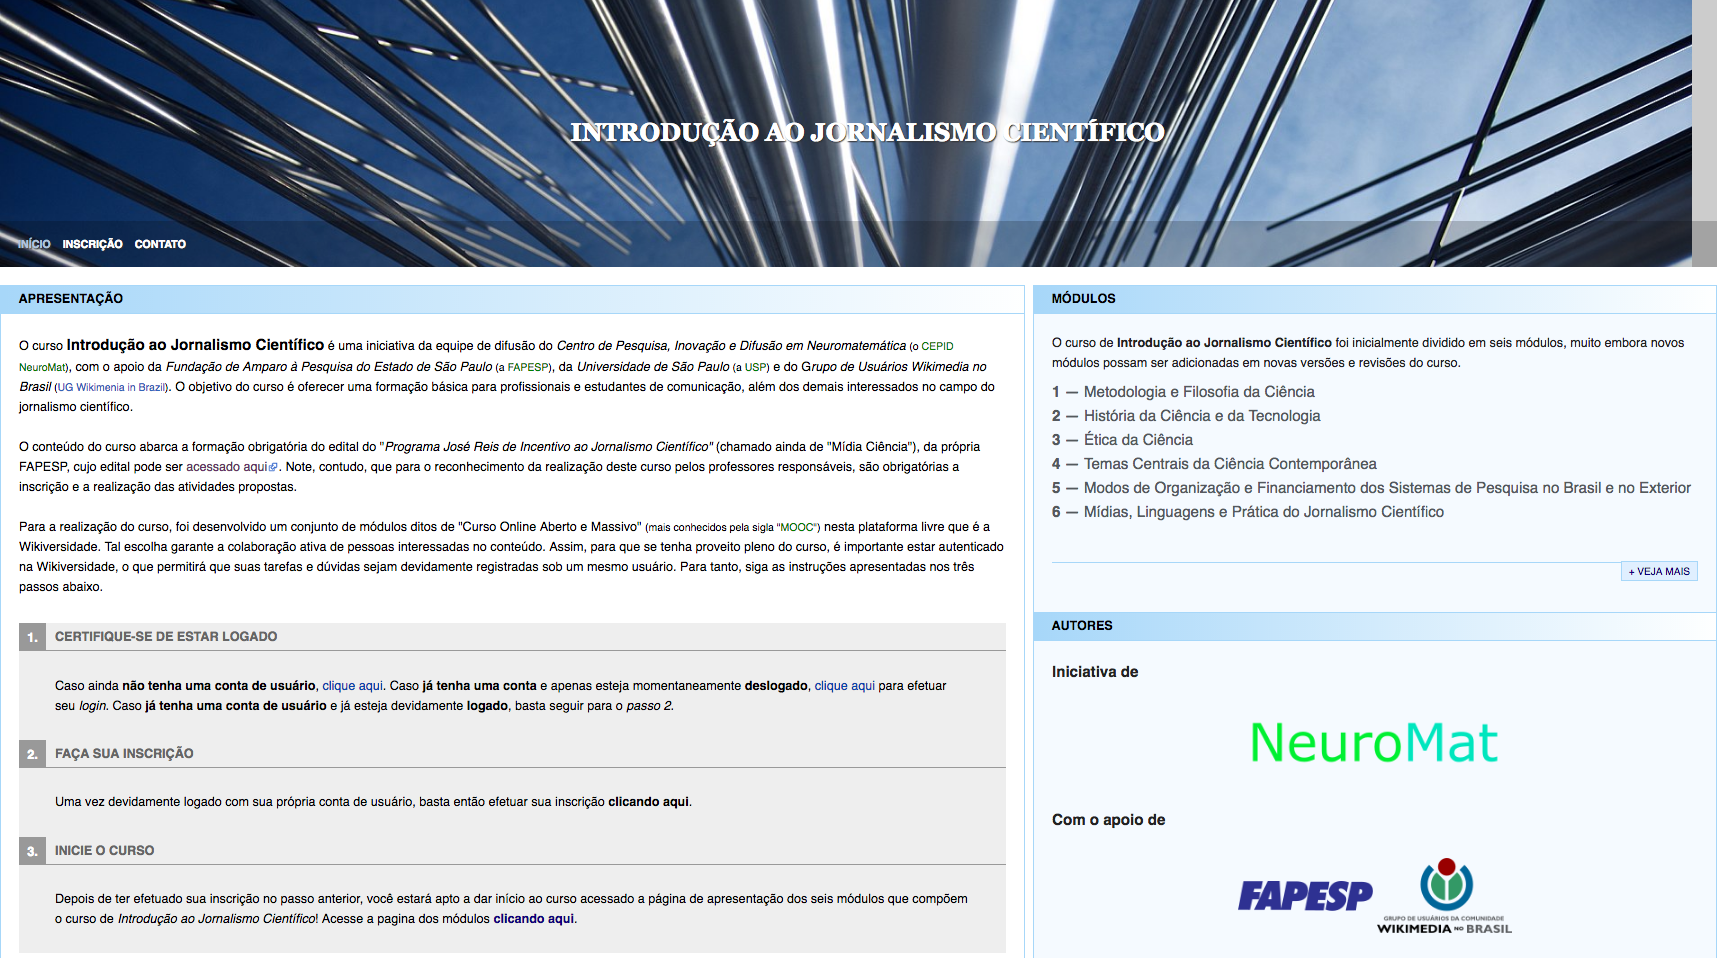
\includegraphics[width=0.9\textwidth]{fig01.png}
\caption{Página inicial do curso Introdução ao Jornalismo Científico.}
\label{fig01}
\source{Wikiversidade.}
\end{figure}

Intitulado de “Introdução ao Jornalismo Científico”, o curso (Ver \Cref{fig01}) teve sua produção iniciada em 9 de maio de 2017. A produção foi coordenada pela equipe de difusão do CEPID NeuroMat e contou com o apoio do grupo de usuários Wikimedia no Brasil, da FAPESP e da Universidade de São Paulo. O desenvolvimento do curso começou pelo conteúdo do Módulo 5, que serviu como piloto, e é chamado de “Modos de Organização e Financiamento dos Sistemas de Pesquisa, no Brasil e no Exterior”. Ele contém 35.644 caracteres, oito imagens de gráficos e mapas, seis vídeos e 13 quizzes, distribuídos pelas seguintes aulas:

\begin{itemize}
\item Panorama mundial dos investimentos em pesquisa e desenvolvimento (Ver \Cref{fig02});
\item Os primeiros financiamentos de P\&D e sua chegada ao Brasil;
\item O estabelecimento da pesquisa no Brasil;
\item A estrutura de financiamento para a ciência no Brasil;
\item As instituições responsáveis pela pesquisa e pela distribuição da verba;
\item Pesquisadores: quem são, onde trabalham e quais as áreas de atuação.
\end{itemize}

\begin{figure}[htbp]
\centering
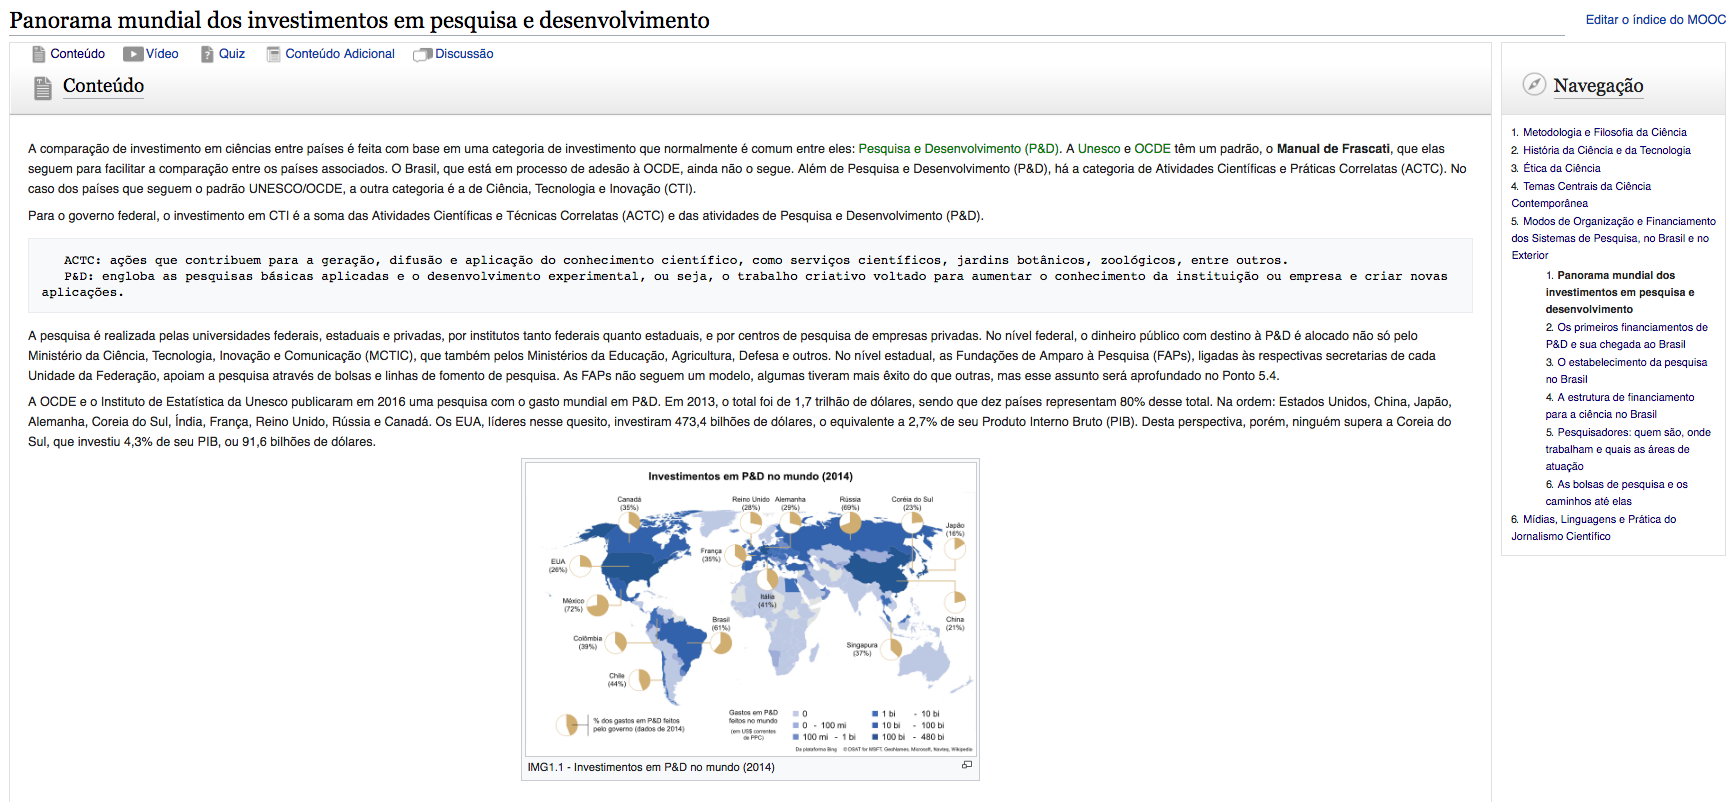
\includegraphics[width=0.9\textwidth]{fig02.png}
\caption{Página da aula inicial do quinto módulo “Modos de Organização e Financiamento de Pesquisas no Brasil e no Exterior”.}
\label{fig02}
\source{Wikiversidade.}
\end{figure}

A programação da página do curso foi um desafio devido à escassez de cursos online de fato na Wikiversidade em português e à necessidade de compreender as linguagens necessárias para escrever os códigos: Lua, JavaScript e CSS. A maioria das páginas da Wikiversidade é, na verdade, ementas e programas de aulas presenciais e grupos de estudo. Então, foi necessário buscar por modelos de cursos nas Wikiversidade em outras línguas. Isso facilitou por um lado, pois programar tudo do zero daria muito mais trabalho do que seguir um modelo. Por outro, foi preciso compreender a linguagem do modelo e ajustá-lo às necessidades do curso. 
Além disso, o código original veio com algumas falhas, como links que não levavam a página alguma. Por exemplo, há a opção de publicar uma pergunta ou comentário para levantar uma discussão no fórum. Ao testá-la, verificou-se que a postagem não aparecia no fórum. O problema veio do código original, elaborado por um curso da Wikiversidade anglófona e, para encontrá-lo e solucioná-lo, foi necessário ir a fundo nas várias linhas de código para entender o caminho construído pelo desenvolvedor (Ver \Cref{fig03}).

\begin{figure}[htbp]
\centering
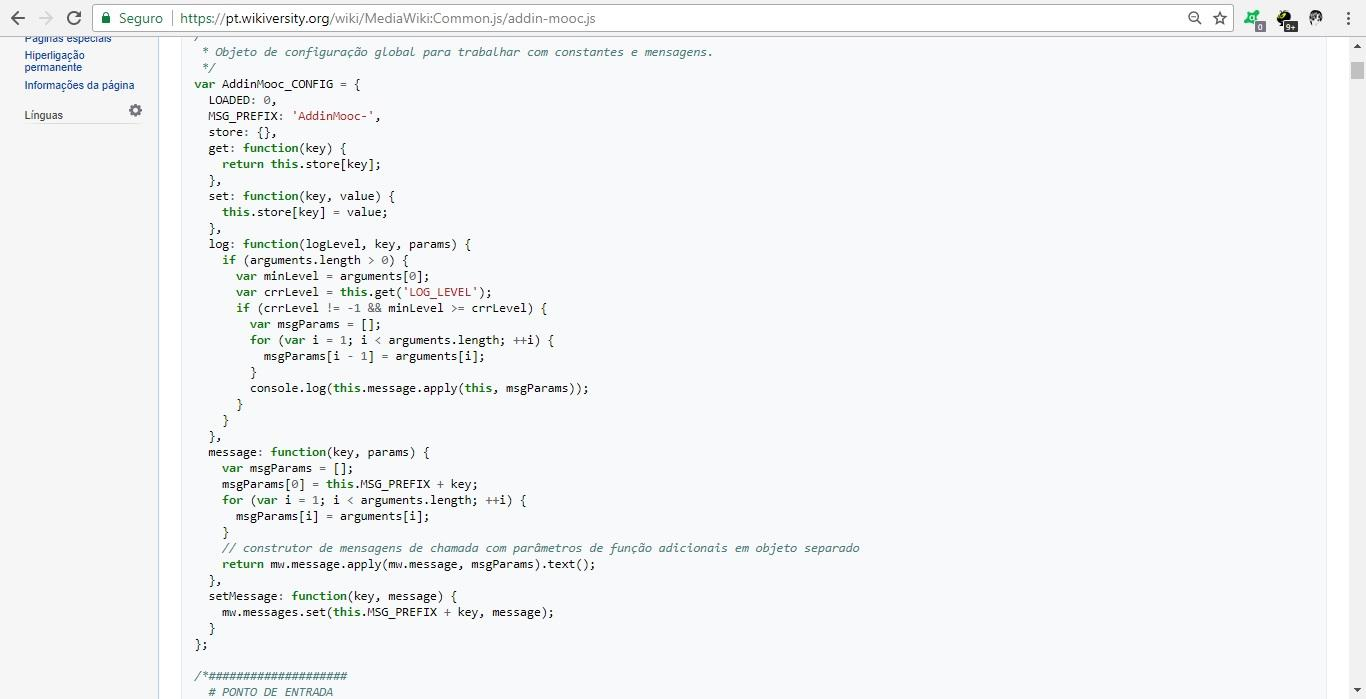
\includegraphics[width=0.9\textwidth]{fig03.png}
\caption{A área de programação da Wikiversidade com parte das linhas de código MediaWiki, base para o funcionamento.}
\label{fig03}
\source{Wikiversidade.}
\end{figure}

Optou-se por não usar apenas texto como conteúdo didático do curso. Isso vai na linha de \textcite[p. 71]{filatro2008} e \textcite[p. 106]{mattar2014}, que consideram o material educativo em formato multimídia como “um dos principais benefícios do aprendizado eletrônico em relação ao aprendizado convencional” \apud[p. 3]{filatro2008,mattar2014}{santo2015}.  
%(apud \cite[p. 3]{santo2015}. 
Em um relato sobre a criação do primeiro MOOC (Massive Open Online Course) da Universidade do Porto, \textcite[s.p.]{martins2016} consideram que “a produção de conteúdo audiovisual de alta qualidade faz de fato a diferença no envolvimento dos formados com o curso”. Para \textcite[p. 26]{cruz2008}, os meios audiovisuais atraem e são tão populares porque têm sua base numa “linguagem complexa, sensorial, que atinge nossa percepção como um todo, de forma gratificante e que deve muito de sua expressão ao cinema”.

Levando em consideração a virtual capacidade dos recursos multimídias e, nomeadamente, do audiovisual para o conteúdo didático, também foram criados vídeos para os módulos. Para tanto, os envolvidos na criação do curso tiveram de roteirizar, produzir, gravar e editar o conteúdo audiovisual. Para os vídeos, foi usada uma técnica chamada de overhead shooting, na qual a câmera posiciona-se acima de uma pessoa, de forma que aparece somente o braço dela, normalmente desenhando. Parte dos vídeos foram produzidos no contexto da bolsa 2016/25810-3, sobre o uso da imagem complexa na difusão científica \cite{ebohon2017}. Um deles, “O que é pesquisa e desenvolvimento”, foi feito com o Videoscribe, um software que permite a produção audiovisual sem que haja uma gravação de fato. Ou seja, o programa usa gravações prévias de overhead shooting, que veem junto com o programa, de uma pessoa escrevendo ou desenhando palavras ou imagens de um banco de dados também do programa. Contudo, o processo é demorado e o resultado, um tanto quanto artificial. Depois, teve início a gravação de vídeos propriamente dito com a técnica de overhead shooting, como no caso do vídeo “Panorama mundial dos investimentos em pesquisa e desenvolvimento” (Ver \Cref{fig04}).

\begin{figure}[htbp]
\centering
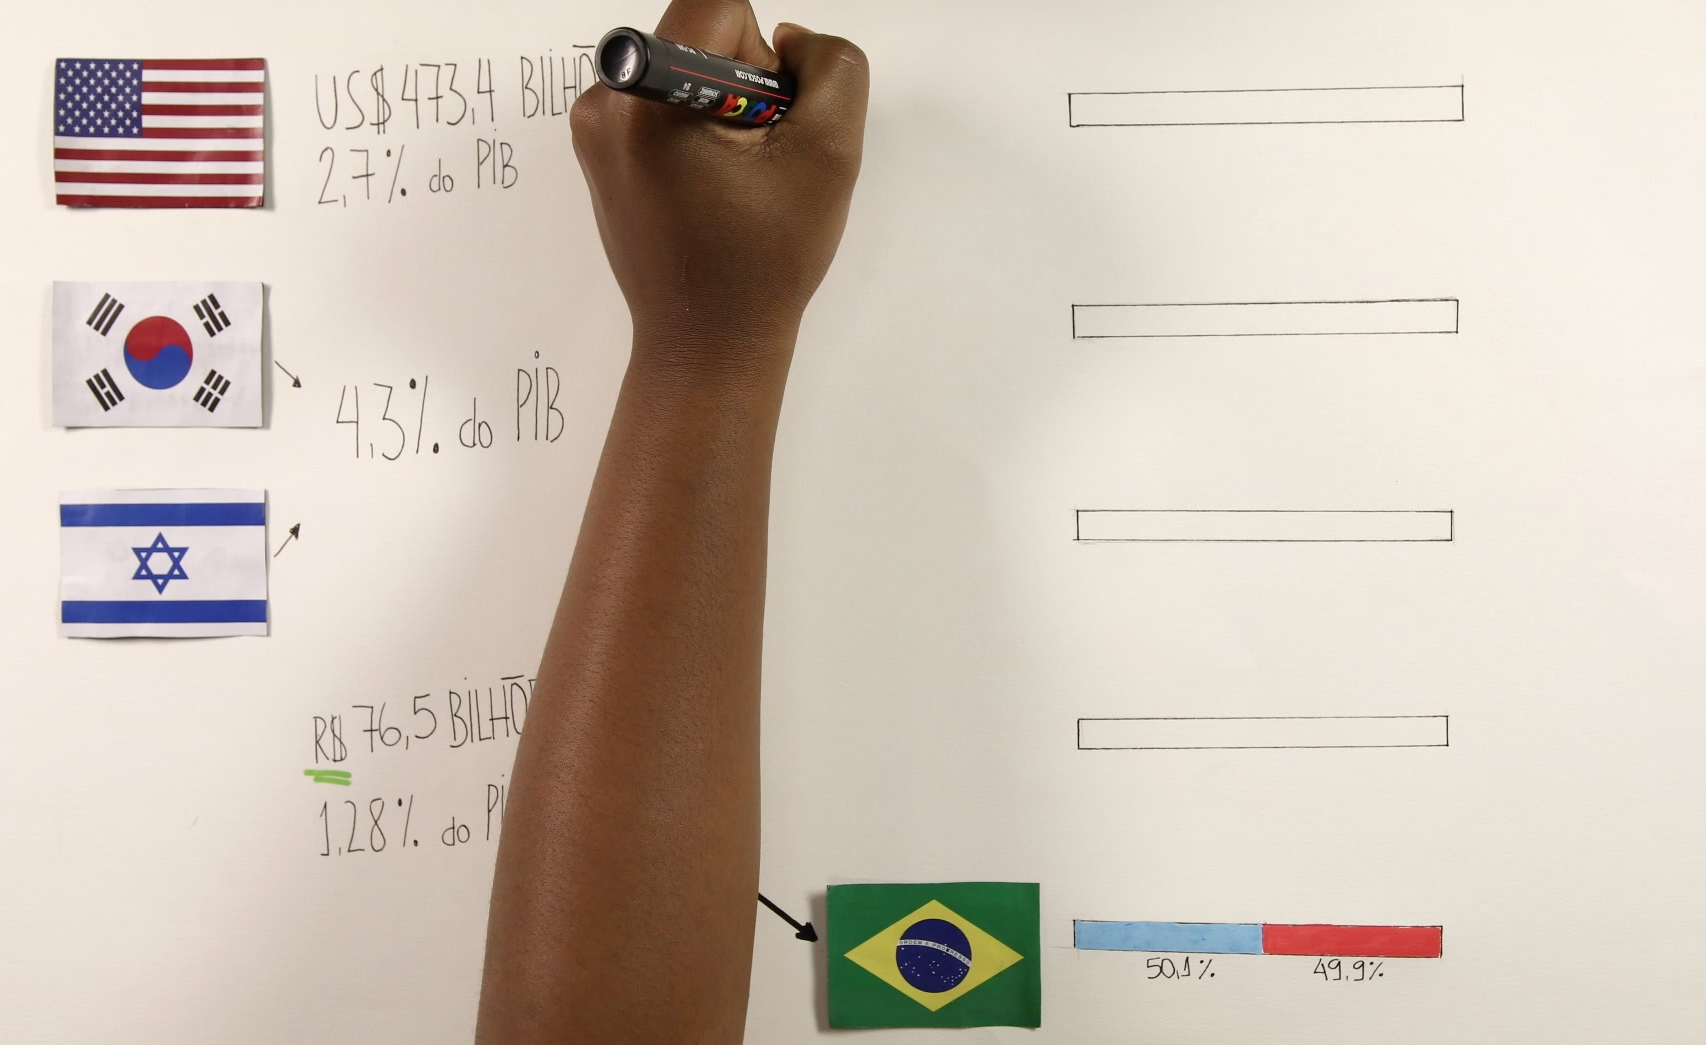
\includegraphics[width=0.7\textwidth]{fig04.png}
\caption{Cena do vídeo “Panorama mundial dos investimentos em pesquisa e desenvolvimento”.}
\label{fig04}
\source{autores deste artigo.}
\end{figure}

Adotou-se o acesso aberto e a licença aberta (CC BY-SA 4.0) para todo o curso, do código usado na programação ao conteúdo didático. Isso porque um dos objetivos não só da Wikiversidade, mas da Fundação Wikimedia, é “liberar o trabalho criativo e cultural das restrições e limitações das leis de copyright” \cite[s.p.]{friesen2008} (tradução nossa). A Fundação Wikimedia também apoia o Wikimedia Commons, repositório que disponibiliza arquivos multimídia (imagens, sons e vídeo) de caráter educativo e/ou pedagógico em licença livre ou em domínio público. Está no Wikimedia Commons, inclusive, o material didático criado para o curso, e que, por causa da licença aberta, pode ser reutilizado para outros fins. Do mesmo modo, é possível adicionar às aulas conteúdos já existentes, de licença compatível com a da Wikiversidade.

Quando uma ferramenta ou um conteúdo é disponível em licença aberta, ela pode ser chamada de Recurso Educacional Aberto (REA). Segundo \textcite[p. 260]{aires2016}, eles são “qualquer tipo de materiais educativos do domínio público ou associados a uma licença aberta” \cite[p. 260]{aires2016}. \textcite[p. 52]{tori2015} sugere que a importância dos REA seja a capacidade de usar, modificar e adaptar conteúdos e mídias, “os quais passam a ficar disponíveis para outros interessados”. No entanto, a criação de um REA pode necessitar de capacidades específicas, como a edição de vídeo. Nessa linha, \textcite[p. 52]{tori2015} afirma que, se “cada professor tiver de desenvolver seus próprios conteúdos, não sobrará tempo para sua atividade fim, além de ser difícil para um professor dominar bem a produção de diferentes mídias”.

Foi feita uma procura por conteúdos de licença aberta e compatíveis com a da Wikiversidade que pudessem ser reutilizados com material para curso Introdução ao Jornalismo Científico. Apesar de menos do que o esperado, a procura trouxe alguns resultados. Foram encontrados conteúdos para algumas aulas em espaços como os blogs Scielo em Perspectiva e Traço de Ciência, mantidos respectivamente pela Rede ScieELO e pelo CEPID NeuroMat, e o SciDev.Net, site jornalístico com foco em ciência e tecnologia para o desenvolvimento global. Da Wikiversidade anglófona, tiramos os templates das caixas seccionais da página inicial (a separação entre “apresentação”, “módulos”, “contato”) e a estrutura dos quizzes, que foram ajustados ao curso (Ver \Cref{fig05}).

\begin{figure}[htbp]
\centering
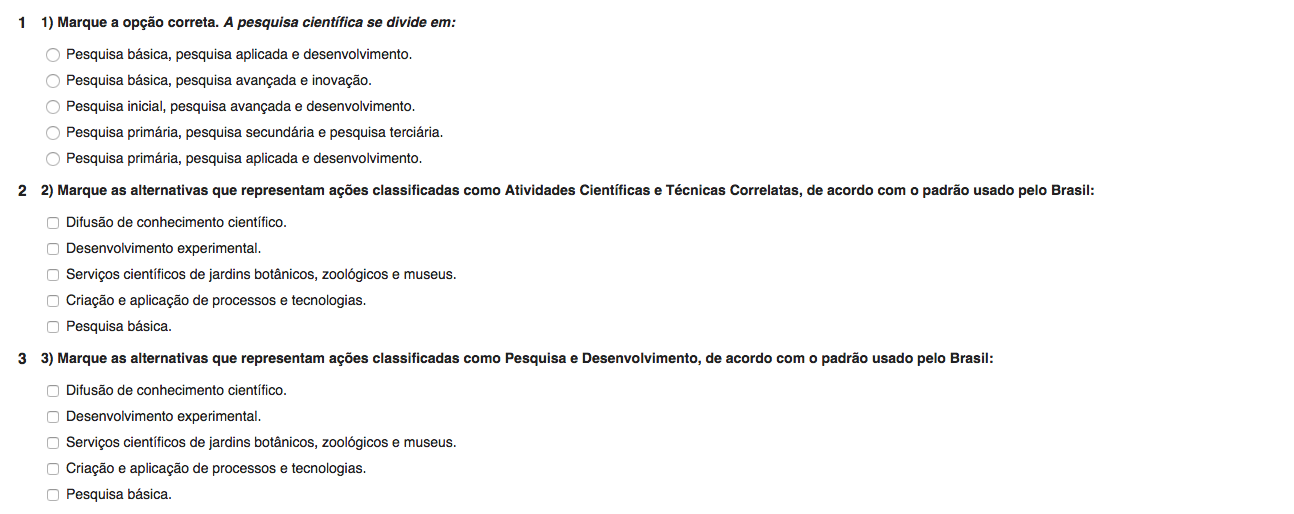
\includegraphics[width=0.9\textwidth]{fig05.png}
\caption{Quiz usado na aula “Panorama mundial dos investimentos em pesquisa e desenvolvimento” do quinto módulo.}
\label{fig05}
\source{Wikiversidade.}
\end{figure}

A despeito de não ser o objetivo deste artigo enquadrar o curso em alguma classificação de ensino online, parece-nos razoável apontá-lo como semelhante aos MOOC, os cursos online abertos e massivos (Massive Open Online Courses). Os MOOC surgem no contexto da Web 2.0 e podem ser vistos como uma modalidade de ensino a distância \cite[p. 185]{forno2013}. \textcite[p. 116]{amiel2015} dizem que esses cursos formam o mais recente movimento a receber o “selo de abertura”. Talvez seja razoável dizer que os cursos abertos são parte da educação aberta, cujas diversas definições têm em comum a remoção de barreiras, segundo \textcite[p. 180]{forno2013}.

Tais barreiras podem ser econômicas e acadêmicas, como a obrigatoriedade em pagar uma taxa de matrícula ou de apresentar algum tipo de certificação acadêmica. Outra barreira é a da exclusividade sobre uma informação. Quando ela inexiste, como no caso dos REA, torna-se viável a “produção baseada em commons”, que usa, de acordo com \textcite[p. 18]{benkler2009}, “insumos de um commons sobre o qual ninguém tem direitos exclusivos, e que libera os seus produtos de volta para o mesmo commons, enriquecendo seus criadores e qualquer um que, como eles, siga os mesmos padrões de produção”. 

Entre os MOOC, há uma divergência de entendimento do conceito “aberto” e, por efeito, em relação à remoção das barreiras, que levou estudiosos a separar os MOOC em dois grupos, cMOOC e xMOOC. Sobre o primeiro grupo, \textcite[p. 6]{teixeira2015} falam que

\begin{quote}
Enquanto os cMOOCs são de natureza conectivista e entendem o conceito de ‘aberto’ tal como este foi definido no campo da educação aberta (OERs, OEPs), os xMOOCs seguem uma abordagem mais tradicional da aprendizagem e entendem ‘aberto’ sobretudo como um sinônimo de ‘gratuito’.
\end{quote}
	
O primeiro MOOC a se chamar assim era de caráter conectivista, tanto que ele se chamava “Connectivism and Connective Knowledge” (Conectivismo e Conhecimento Conectivo) e foi oferecido por George Siemens, Stephen Downes e Dave Cormier na Universidade de Manitoba, no Canadá, em 2008 \cite[p. 5]{teixeira2015}. O segundo grupo, dos xMOOC, é definido por \textcite[p. 185]{forno2013} como de linha “behaviorista”, e “os modelos xMOOCs correspondem, fundamentalmente, a uma extensão dos modelos pedagógicos utilizados pelas instituições de ensino tradicionais, privilegiando, porém, as práticas instrucionais de ensino, ou seja, fazendo uso do design instrucional”. Tendo em vista os dois conceitos e as características dos wiki, talvez seja possível dizer que o curso de jornalismo científico tenha traços do conectivismo do cMOOC.

Conceituado por \textapud{siemens2004,siemens2006}[p. 363]{alevizou2017} o conectivismo é uma abordagem que mescla noções de educação aberta e ensino a distância com teorias de rede. A ideia por trás dos cMOOCs é que os estudantes participem de um processo educativo colaborativo, no qual eles possam trocar informações por meio das conexões em rede. De acordo com \textcite[p. 365]{alevizou2017}, a hipótese do conectivismo é que ele 

\begin{quote}
pode promover um sentido coletivo de responsabilidade e orgulho, contribuindo para uma cultura mais auto-reflexiva e proporcionando um impulso para o pensamento e a criatividade [...]. Nesse modelo, o conhecimento é construído a partir da mediação cultural e com base em uma pedagogia construtivista fundamentada na ideia de aprender fazendo e  avaliação por pares.
\end{quote}.
	
“Aprender fazendo” e “avaliação entre pares” são duas das características apontadas por \textcite{lawler2008} e \textcite{lai2009} quando usa-se tecnologia wiki para o aprendizado, ou para o wikilearning de \textcite{suoranta2015}. O curso Introdução ao Jornalismo Científico mostra traços de conectivismo porque ele tende à abertura em termos de acesso e licença e, por efeito, permita que o usuário arquitete as aulas como bem entender e veja o caminho percorrido por outro usuário ao longo das aulas. Ademais, \textcite{junior2017} apontam como característica dos wiki para a educação online a estruturação de “comunidades de aprendizagem”, possibilidade esta que \textcite{lawler2008} diz ser um dos “propósitos” de existir da Wikiversidade. 

Colocar um tema central, ao redor do qual pode ser criado uma comunidade de aprendizagem, talvez incentive uma maior conectividade entre as pessoas envolvidas. Nesse sentido, \textcite[p. 180]{gomes2011} relatam que, durante uma atividade de ensino de jornalismo com ferramentas wiki, o estabelecimento de um mesmo tema a ser abordado trouxe mais conectividade entre os alunos e entre os grupos. Contudo, não se engendrou uma comunidade de aprendizagem em torno de um assunto, o jornalismo científico, para além dos sete integrantes da equipe de difusão do CEPID NeuroMat que participaram do desenvolvimento do curso. 

Resultou em pouco impacto a estratégia de separar as aulas por assuntos e convidar pessoas, com base nos respectivos históricos profissionais, para contribuir com conteúdo para o curso. Talvez tenha faltado sinergia para o sucesso de certas ações como, por exemplo, o esforço em reativar a Associação Brasileira de Jornalismo Científico. Ela seria a responsável pela certificação de conclusão do curso e poderia contribuir para a estruturação de uma comunidade de aprendizagem na qual, porventura, seriam misturadas gerações de pessoas de diversas áreas interessadas no jornalismo científico e, mais amplamente, na divulgação científica.

Previa-se, no plano inicial, desenvolver totalmente as 90 horas/aula requisitadas pela FAPESP, distribuídas igualmente pelos seis módulos, cada um subdividido em ao menos cinco aulas. Contudo, o período de nove meses não foi suficiente para a alcançar essa expectativa. Em uma ponderação sobre o planejado e o realizado, pode-se dizer que, se não atingimos a expectativa de desenvolver totalmente o curso Introdução ao Jornalismo Científico com conteúdo textual e audiovisual, ao menos foi explorado o lado criativo do desenvolvimento de um curso wiki, do design da página da Wikiversidade à linguagem audiovisual produzida. 

\section{Considerações finais}\label{sec-consideracoes}

O presente artigo apresentou uma revisão bibliográfica e um relato de caso sobre a elaboração do curso Introdução ao Jornalismo Científico. Espera-se, talvez, colaborar para o esclarecimento de conceitos relacionados à educação a distância, como Web 2.0, wiki, conectivismo e MOOC. Os desdobramentos apresentados no relato e as diferenças entre o planejado e executado também podem servir como um suporte para futuros projetos que queiram criar um curso na web, com ferramentas wiki ou não, e inclusive para pessoas que queiram contribuir para a expansão do curso. 

Feitas as considerações sobre a construção do curso Introdução ao Jornalismo Científico, é razoável supor que uma comunidade de aprendizagem pode explorar o aspecto colaborativo dos softwares wiki e a estrutura do curso hospedado na Wikiversidade. No sentido de desenvolver uma comunidade de aprendizagem, o conectivismo porventura pode ser uma abordagem possível. Ao descrever a aula sobre conectivismo criada por Siemens, Downes e Cormier, na qual colocou-se em prática os princípios do conectivismo, \textcite[p. 5]{teixeira2015} dizem: 

\begin{quote}
o conteúdo resultou da produção de artefactos pelos participantes [...], os organizadores atuaram mais como facilitadores e fornecedores de alguma estrutura necessária, sendo a função de “ensinar” atribuída à própria comunidade de aprendizagem.
\end{quote}
	
É destacado que os primeiros participantes do curso Introdução ao Jornalismo Científico foram os sete integrantes que atuaram, de alguma maneira, em sua criação. Se uma página wiki pode ser aperfeiçoada constantemente, um curso wiki também pode \cite[p. 93]{zhang2009}. Esse cenário, em conjunto com as práticas do conectivismo de aprender fazendo e entre pares, parece-nos propício de acontecer se uma comunidade de aprendizagem for estabelecida, algo que talvez seja viável se tomado como base o programa Mídia Ciência. Embora o público-alvo do curso seja qualquer pessoa interessada em jornalismo científico, dado o aspecto aberto e livre do curso, é concebível pensar que jornalistas e/ou proponentes ao programa da FAPESP são grupos talvez mais propensos a participar do curso.

Uma sugestão para o contínuo aprimoramento do curso de introdução ao jornalismo científico e, por efeito, a estruturação de uma comunidade de aprendizado, seria acrescentar como opção ao proponente do programa Mídia Ciência que ele colabore com conteúdo para o curso. O material acrescido poderia ser avaliado por outros pesquisadores, e o proponente poderia melhorar o conteúdo existente. Aprender fazendo e avaliação entre pares, portanto. Tais práticas auxiliam a construção do conhecimento, para a qual a conectividade entre alunos é fundamental \cite[p. 173]{gomes2011}. Poderia surgir, assim, uma rede pessoas de ligadas ao jornalismo científico e, mais amplamente, à divulgação científica, o que talvez ampliasse a colaboração nesse campo. 

Em entrevista à Universidade Federal de Minas Gerais (UFMG) para falar sobre o estudo “Diagnóstico de la Divulgación de la Ciencia en América Latina”, que participou junto de \textcite{barba2017}, Luisa Massarani diz que “uma das conclusões de nosso estudo sobre a divulgação científica na América Latina é justamente esta: colaboramos muito pouco”. Uma comunidade de aprendizagem colaborativa, constituída não só mas principalmente por pesquisadores do programa José Reis de Incentivo ao Jornalismo Científico, talvez possa contribuir para reverter o diagnóstico de pouca colaboração na área da divulgação científica do Brasil.

\section{Financiamento}\label{sec-financiamento}
A pesquisa teve apoio da FAPESP (processo 2017/05969-0) e do Centro Interdisciplinar de Pesquisa da Faculdade Cásper Líbero.

\printbibliography\label{sec-bib}
% if the text is not in Portuguese, it might be necessary to use the code below instead to print the correct ABNT abbreviations [s.n.], [s.l.] 
%\begin{portuguese}
%\printbibliography[title={Bibliography}]
%\end{portuguese}



\end{document}
